\documentclass[11pt]{article}

% --- packages (same set as the pilot paper, dsls-as-harnesses) ----------------
\usepackage[utf8]{inputenc}
\usepackage[T1]{fontenc}
\usepackage[margin=1in]{geometry}
\usepackage{microtype}
\usepackage{amsmath}
\usepackage{booktabs}
\usepackage{array}
\usepackage{needspace}
\usepackage{graphicx}
\usepackage{xcolor}
\usepackage{listings}
\usepackage{tikz}
\usetikzlibrary{arrows.meta,positioning,calc,fit}
\usepackage[numbers,sort&compress]{natbib}
\usepackage[colorlinks=true,allcolors=blue]{hyperref}

\definecolor{codebg}{gray}{0.96}
\lstset{
  basicstyle=\ttfamily\footnotesize,
  backgroundcolor=\color{codebg},
  frame=single,
  framesep=4pt,
  rulecolor=\color{gray!40},
  breaklines=true,
  columns=fullflexible,
  keepspaces=true,
  showstringspaces=false,
  aboveskip=1em,
  belowskip=1em,
}

\title{\textbf{The Harness Is the Language:\\ When Everyone Writes Software and No One Reads It}}

\author{
  Satoshi Nakajima\\
  \small The Singularity Society\\
  \small \texttt{satoshi@singularitysociety.org}
}

\date{5 September 2026}

\begin{document}
\maketitle
\let\thefootnote\relax\footnotetext{\copyright\ 2026 Satoshi Nakajima. This work is
licensed under a Creative Commons Attribution 4.0 International (CC BY 4.0) license:
\url{https://creativecommons.org/licenses/by/4.0/}.}

\begin{abstract}
Most software is written for many people and used many times, and every practice we have for making it safe assumes that scale. A growing share of software is now written for one person, or for a few dozen, and used for a week or a season and then set aside: software whose $N$ is too small to pay for a reader; it exists because an AI can write it in minutes, and it is only worth writing because writing it is nearly free. Such software has no budget for review and no budget for a second version, and if the AI that wrote it is trusted with everything, then everything the AI gets wrong is shipped.

We propose a single design move for this class of software: draw a line through the application and let the AI's freedom differ on either side. Above the line sit the view and the UI controller, the part that decides what to show and what to ask for; there the AI writes ordinary code with no restriction. Below the line sit the model and the business logic, the schema, the state transitions, the permissions, and the integrity of the data; there the AI does not write imperative code, which is hard to verify. It writes a \emph{declaration} in a small language whose vocabulary is finite and whose every sentence has one meaning, and the declaration is checked mechanically and enforced outside anything the AI wrote. Code above the line can only \emph{ask}; the declaration below it \emph{decides}.

The language below the line is designed for an AI rather than for a programmer. Where a language for people competes on expressiveness, a language for an AI competes on what can be verified about a program before it runs, and it gives up computation to get it. This makes the language itself the harness: instead of inspecting what the AI produced, or confining it at run time, the language settles in advance what the AI is able to say.

We present the principle, the properties such a language must have, and one instance: a platform on which twenty-six shared web applications have been produced from prompts alone, with no line of declaration or page edited by hand, from surveys and booking sheets to a public forum where AI agents argue under rules that none of them can break, and that their host can change only by changing the declaration. We report how the language's vocabulary grew under use, what the line protects, and what it deliberately does not.
\end{abstract}

\noindent\textbf{Keywords:} AI-generated software; small-$N$ software; declarative authorization; domain-specific languages; harnesses for language models; end-user software engineering.

\section{Introduction}
\label{sec:intro}

Software engineering is organized around a denominator. A program is expensive to write, so it must be used by enough people, enough times, to pay for itself; every practice that keeps software safe---code review, test suites, staged deployment, on-call rotation---is affordable only because that denominator is large. Call the number of people who will ever use a program its~$N$. Almost everything we know about building software well was learned at large~$N$. $N$ is a deliberately simple proxy for the economic denominator of a program: how long it will live, how often it will run, and what a failure would cost all enter that denominator too, and a program used by five people every day for twenty years to move money is not what is meant here. ``Small-$N$'' in this paper names software whose expected use is too small to pay for anyone to read it, whatever the count of its users happens to be.

Large language models have changed the cost side of that equation. A working web application that would have taken a developer a week can now be produced in an afternoon by someone who has never written code, by describing it to an AI. That does not make large-$N$ software cheaper by much: the cost of that software was never mostly in the writing. What it does is make a new kind of software possible: software with a small~$N$. A sign-up sheet for one workshop. A booking form for one gym class. A survey for one talk, answered by eighty people over a weekend and then forgotten. Such software could not exist before, because no one could justify writing it. Now it can be written for the cost of asking.

Small-$N$ software has properties that large-$N$ software does not. It has no budget for review: nobody is going to read the code of a form that eighty people will use for a weekend. It has no budget for a second version: if it is wrong, nobody is coming back to fix it, and the people who used it have already been served wrong. And it is written by an AI whose author, very often, cannot read what was written. So the question of how much to trust the AI is not a matter of taste. Whatever the AI is trusted with, it is trusted with completely, because nothing else is looking.

Two answers are current. One is to trust the AI with everything and manage the consequences afterwards. This is the shape of the prompt-to-app products~\cite{vibetools2026} and of what ``vibe coding''~\cite{karpathy2025vibe} names: the AI writes the whole application, front end, back end and data model, in the same open-ended languages, and the safeguards come after the fact---generated tests, static analysis, a policy linter, a scan before publishing, a second AI reviewing the first, a sandbox and a permission prompt. The other is to trust it with nothing that matters, and confine it to producing what a person could have produced with a form builder. The first answer inspects the output of a process that was allowed to produce anything; the second forbids the process from producing much. Neither is a good fit for software that has no second version and no reader.

This paper proposes a third answer, and it is a single move: \emph{draw a line}. Split the application into the part where the AI's errors are cheap and the part where they are not, and let the AI's freedom differ on the two sides. Above the line, the AI writes code as it pleases. Below the line, it writes in a language built so that what the AI can say is exactly what can be checked: a declaration, not a procedure. The line is not a boundary between two components of a program. It is a boundary between two \emph{policies} for one AI.

The change of author is what changes the design of the language below the line. For a human author, expressiveness is a virtue, and a language is judged by how much a skilled person can say in it. For an AI author whose output will not be read, expressiveness is also attack surface: every construct the language admits is a construct the AI may use wrongly with nobody to notice. So the language below the line is designed to a different target, what can be known about a program before it runs rather than what can be said in it, and that is what makes the language a harness.

The contributions are:
\begin{itemize}
\item The line: risk-proportional freedom for one AI author, with the view and UI controller above it and the model and business logic below, so that the generated page is untrusted and the generated declaration is not (\S\ref{sec:line}).
\item The closed interface across the line: a small set of intents, so that the freedom above the line is genuinely free because nothing above it is consulted when a request is judged (\S\ref{sec:above}).
\item Enforcement that outlives the author's machine and binds strangers, including ones who bypass the page, because the declaration is projected onto a system outside anything the AI wrote (\S\ref{sec:language}, \S\ref{sec:instance}).
\item The properties the language below the line must have for the above to hold, and the argument that such a language is a harness in itself (\S\ref{sec:language}).
\item An instance: a platform on which twenty-six shared applications were built and published from prompts alone, listed in Appendix~\ref{sec:appendix}, and a record of how the language's vocabulary grew under that use (\S\ref{sec:instance}).
\item An account of what the line protects and what it leaves alone (\S\ref{sec:limits}).
\end{itemize}

\section{Drawing the Line}
\label{sec:line}

Consider a program as four parts, following the classical model--view--controller separation~\cite{krasner1988mvc} with the model split into data and rules. The \emph{view} draws the screen. The \emph{UI controller} decides what the screen shows next and what the user is being asked to do. The \emph{model} holds the data and its shape. The \emph{business logic} decides what the data is allowed to become: which records may exist, who may create them, which state follows which, and what may never be undone.

An error in each part costs a different amount. A view that draws a button in the wrong color is noticed and forgiven. A controller that shows the confirmation screen before the form is annoying. A model that lets two people book the same seat, or a business rule that lets a stranger delete somebody else's record, is not an inconvenience; it is a breach, and in small-$N$ software there is no one to catch it. The four parts differ not in how hard they are to write but in how much a mistake in them costs.

The line goes between the second part and the third. Above the line are the view and the UI controller: everything about \emph{what to show and what to ask}. Below it are the model and the business logic: everything about \emph{what is true and what is permitted}.

\begin{figure}[tb]
\centering
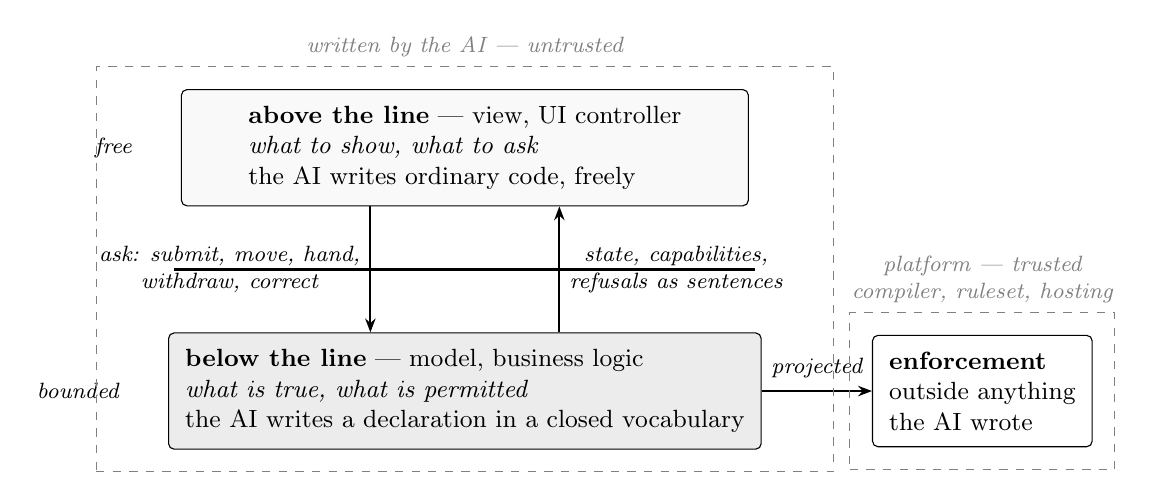
\begin{tikzpicture}[
  box/.style={draw, rounded corners=2pt, align=left, inner sep=6pt, font=\small},
  lab/.style={font=\footnotesize\itshape, align=center},
  arr/.style={-{Stealth[length=5pt]}, thick}
]
\node[box, minimum width=7.2cm, fill=gray!5] (above) {
  \textbf{above the line} --- view, UI controller\\
  \emph{what to show, what to ask}\\
  the AI writes ordinary code, freely};
\node[box, minimum width=7.2cm, fill=gray!15, below=1.6cm of above] (below) {
  \textbf{below the line} --- model, business logic\\
  \emph{what is true, what is permitted}\\
  the AI writes a declaration in a closed vocabulary};
\draw[very thick] ($(above.south west)!0.5!(below.north west)$) -- ($(above.south east)!0.5!(below.north east)$);
\draw[arr] ([xshift=-1.2cm]above.south) -- ([xshift=-1.2cm]below.north) node[midway, left, lab] {ask: submit, move, hand,\\ withdraw, correct};
\draw[arr] ([xshift=1.2cm]below.north) -- ([xshift=1.2cm]above.south) node[midway, right, lab] {state, capabilities,\\ refusals as sentences};
\node[box, right=1.4cm of below, fill=white, align=left] (enf) {\textbf{enforcement}\\ outside anything\\ the AI wrote};
\draw[arr] (below) -- node[above, lab, yshift=1pt] {projected} (enf);
\node[lab, left=0.5cm of above] {free};
\node[lab, left=0.5cm of below] {bounded};
\node[draw, dashed, gray, inner xsep=26pt, inner ysep=8pt, fit=(above)(below), label={[lab, gray]above:written by the AI --- untrusted}] {};
\node[draw, dashed, gray, inner sep=8pt, fit=(enf), label={[lab, gray, align=center]above:platform --- trusted\\ compiler, ruleset, hosting}] {};
\end{tikzpicture}
\caption{The line. The AI's freedom differs on the two sides. The page above can only ask, through five intents; the declaration below decides, and it decides through enforcement that neither the page nor the AI can bypass. Everything the AI writes is untrusted; what is trusted is the platform that reads the declaration (\S\ref{sec:projection}).}
\label{fig:line}
\end{figure}

Two policies then follow. Above the line, the AI is free. It writes the page in whatever language and style it likes, draws whatever it wants, and arranges the screens as it sees fit. No check is run on this code beyond the ordinary ones, and none is needed, because nothing this code does can change what is true below the line. If it is wrong, the page looks wrong.

Below the line, the AI is not free. What it writes there is not a procedure, which is hard to verify, but a \emph{declaration}: a document in a small language with a fixed vocabulary, saying what the records are, who may write them, how their state moves, and what holds them together. The declaration is checked mechanically before anything is published, and once published it is enforced by a system that neither the page nor the AI that wrote the declaration can reach around.

What connects the two sides is the crucial design decision. Code above the line cannot reach into the data. It can only \emph{ask}: submit this, move this record to that state, hand this row to that person, withdraw this, correct these fields of this. What it can ask for is a small closed set of intents, and whether any request is honored is decided entirely by the declaration. The page proposes; the declaration disposes. In this way the freedom above the line is genuinely free---the AI can write anything, and what it writes cannot cause a change to the data that the declaration does not permit. It can still ask for a permitted change that the person did not intend, and it can draw the wrong screen; what a wrong page can do to the person using it is another matter, and \S\ref{sec:limits} returns to it. What the line guarantees is integrity with respect to the declared policy, not that the application is right.

This is what distinguishes the line from ordinary layering. Model--view--controller and the three-tier architecture separate concerns so that people can work on them independently; every layer is still code, written by the same kind of author under the same trust. The line separates \emph{trust}. The two sides are written by the same AI in the same session, and the difference between them is what the AI is permitted to produce. Above, anything. Below, only sentences the language can check.

\section{Below the Line: A Programming Language for AI}
\label{sec:language}

The declaration below the line is a program, and the language it is written in is a language for writing programs. It is not one a programmer would recognize as such: it has no way to compute. That is not an omission but the design, because the language is written for a different author, and that changes what a language is for. A language for an AI should compete on verifiability rather than on expressiveness, and if that makes it a closed configuration language rather than a general one, that is the price, paid deliberately.

A language for programmers competes on expressiveness. It should let a skilled person say what they mean concisely, compose small things into large ones, and reach for the general case when they need it. Escape hatches are a virtue: when the language cannot express something, a programmer wants a way out.

A language for an AI competes on something else: on how much can be known about a program before it runs, by someone who did not write it and will not read it. The author is not a person to be trusted and empowered but a process to be bounded. That reverses several instincts.

\paragraph{The vocabulary is closed.} There is a finite list of things that can be said, and nothing else. There is no escape hatch, no general-purpose expression, no way to compute. The absence of a way out is the point: every program in the language is drawn from a set whose members are known, and a checker that understands each member understands every program.

\paragraph{Each sentence has one meaning.} A declaration is read by the AI that writes it, by the checker that validates it, by the enforcement system that projects it, and, when something is refused, by the person who wants to know why. It is written with one meaning so that all four read the same thing. \texttt{sealed: ["closed"]} means that a record in the closed state cannot be deleted, by anyone, including the owner; it does not mean anything else, and there is nothing in it to be interpreted.

\paragraph{Refusal returns to the declaration.} When an operation is refused at run time, the reason is a sentence of the declaration: this move is not in the transition table; this record refers to one that is no longer open; this field was stamped by the server and cannot be rewritten. The person who asked can be told which sentence refused them, and it is a sentence they can read. This is only possible because the language is closed: an arbitrary program refuses for arbitrary reasons.

\paragraph{The meaning of a declaration is independent of its enforcement.} A declaration says what must hold, not how it is checked. It names no database, no rule engine, no server, and each sentence means the same thing whatever will enforce it. This independence is narrower than it sounds, and the instance in \S\ref{sec:instance} shows exactly how: the \emph{meaning} of a sentence does not depend on the target, but which sentences exist, and the shape they take, has so far been decided with one target in view (\S\ref{sec:projection}). Until a second projection exists, the claim is that the vocabulary could be projected elsewhere, not that it was designed without a target in mind.

\paragraph{Enforcement lies outside what the AI wrote.} A declaration says what must hold; something else holds it. That something is not the page, not the AI, and not any code either of them produced: it is a system that reads the declaration and refuses what the declaration does not allow, wherever the request came from. Without this the closed vocabulary would be a convention, and a page that chose to ignore it would be free to. With it, nothing above the line can violate a declared invariant, because nothing above the line is consulted when a request is judged.

\paragraph{Checking covers the whole language and happens before publication.} Because the vocabulary is closed, the checker covers every sentence the language admits rather than sampling a program's behavior; it is exhaustive with respect to the language's well-formedness conditions, and it is those conditions, not the author's intent, that it decides. It asks every question it has about every declaration: does every referenced collection exist, is every field named in the write list a field that may be written by a stranger, does every state named in a transition exist, does the identity of a record depend on something the submitter controls. A declaration that fails is refused before it is published, and the reason is again a sentence.

Together, these properties make the language a \emph{harness}. The word is usually applied to what surrounds an AI: the sandbox it runs in, the tests run on its output, the reviewer that reads its work, the prompt that asks it to be careful. All of these operate on a process that was allowed to produce anything, and try to contain what it produced. A closed language operates earlier. It decides what the AI is able to produce, so that the question of containing it does not arise. Below the line there is nothing to contain in that sense: what the AI can write there is a declaration, and a declaration is read in full before publication, not a procedure whose effect has to be discovered. What the checker catches is precisely bounded, and it is worth being exact about it. It refuses a declaration that is ill-formed---a transition into a state that does not exist, a stranger allowed to set a record's own status, a role that grants nothing. It cannot refuse a declaration that is well-formed and wrong, one that grants a permission the author did not mean to grant, because nothing in the declaration says what was meant. What the line guarantees is that whatever the declaration says is what will be enforced; whether the declaration says the right thing is a question about the specification, and it remains one (\S\ref{sec:limits}).

This is why the instincts reverse. An escape hatch would be an unbounded region inside the harness. A general expression would be a program the checker cannot finish reading. A sentence with two meanings would be a refusal that cannot be explained. What makes the language poor for a programmer is exactly what makes it a harness for an AI.

\section{Above the Line: Freedom with a Closed Interface}
\label{sec:above}

If the language below the line is closed, the code above it must be genuinely free, or the line has bought nothing. The freedom is real: the page is ordinary HTML, CSS and JavaScript, and the AI writes it as it would write any page. What makes that freedom safe is the interface across the line.

The interface is a small set of \emph{intents}. A page may submit a new record, move an existing record to another state, hand a record to a named person, withdraw a record, or correct the fields of a record it is allowed to correct. Five verbs. Three of them cannot name a field at all; the two that carry values are bounded by the declaration, which lists which fields a submitter may set and which are frozen. There is no sixth verb, and there is no way for the page to write to the data other than through these five.

Each intent is a request, not an action. The page says what it would like; the parent that hosts it forwards the request; the enforcement system decides. A page that asks to reopen a closed topic is refused, and the refusal returns a sentence of the declaration. The page can then say whatever it likes about the refusal, but it cannot get around it, because it has no other way in.

The page is also confined in the ordinary way---it runs in an isolated frame with no network of its own, no form submission or navigation to another origin, no pop-up windows, no way to reach the host it is embedded in except through the intent channel---but this confinement is secondary. Its purpose is to make the intent channel the \emph{only} channel. Once that is so, the question ``what can this page do to the data?'' has a short answer: it can ask for five things, and every one of them is decided elsewhere.

Two consequences follow for how such a page is written, and they are worth stating because they are where a freely written page most often goes wrong. First, a page should draw only from the state it is given, never from what it remembers having asked for: a submission that was cancelled, or refused, must not be drawn as if it succeeded, and the only way to guarantee that is to draw from the data. Second, a page cannot know whether an intent will be honored, only ask; so the capabilities the page is told it has---which transitions this viewer may perform, which fields are frozen---come from the declaration, and a page that draws controls from anywhere else draws controls that do not work. Neither of these is a rule the platform enforces on the page. They are how a page has to be written when it can only ask.

\section{One Instance}
\label{sec:instance}

The line has been drawn in one system, the shared-app platform of MulmoTerminal, an open-source terminal for AI coding agents.\footnote{\url{https://github.com/receptron/mulmoterminal}; the declaration compiler is the \texttt{@receptron/sharedapp} package and the enforcement rules live in the server repository, which is not yet public.} It is a platform for \emph{shared apps}, small web applications built inside an AI coding session and published to a URL, where they are used by people who never see the code. The author describes what they want; the AI writes the page (above the line) and the declaration (below it); a tool checks the declaration and projects it onto the security rules of a hosted document database; and the result is a page that keeps working after the author's machine is gone.

Between 14 August and 1 September 2026 this platform produced twenty-six such apps, all of them built by the platform's author, and every one of them from prompts alone. ``From prompts alone'' is a working rule rather than a measurement: the author's practice was to describe the app and its changes in conversation and never to open the declaration or a page in an editor, and the platform writes both files only through the agent. It is not established by tooling, and the platform does not yet record it. The apps are listed one per row in Appendix~\ref{sec:appendix}, with their sizes, the agent that wrote each, the vocabulary each uses, and a public address for the twenty-three that have a page anyone may open; Table~\ref{tab:apps} groups them by kind. None of them is large: the longest declaration is 157 lines of JSON, the shortest 21, and the median 74. The pages are ordinary HTML and, counted in lines, are about seven times the size of the declarations they sit on (14{,}341 lines against 2{,}111). The apps were written by four different coding agents---Claude Code (22 apps), Grok (2), Codex (1) and Muse (1), recorded per app in Appendix~\ref{sec:appendix}---using the same declaration language. The four apps not written by Claude Code are too few to support a comparison and are listed only to show that the vocabulary is not tied to one agent, which is the first thing to note about a closed vocabulary: it is a contract with whichever model is on the other side, and nothing in it is specific to one.

\begin{table}[tb]
\caption{The twenty-six apps grouped by what they are for. The last column names the sentences \emph{characteristic} of each group's business logic, not the full vocabulary each declaration uses; Appendix~\ref{sec:appendix} has that per app.}
\label{tab:apps}
\centering
\small
\begin{tabular}{@{}lrp{9cm}@{}}
\toprule
kind & apps & characteristic sentences \\
\midrule
survey, sign-up, quiz & 5 & \texttt{public.submit}, \texttt{idFrom}, \texttt{stampField} \\
live poll & 3 & \texttt{transitions} (draft/open/closed), \texttt{live} \\
booking with slots & 4 & \texttt{window.fromField}, \texttt{mirror}, \texttt{selfDelete} \\
task and claim boards & 7 & \texttt{uidField}, \texttt{idIn}, \texttt{selfTransitions} \\
forum, chat, council & 3 & \texttt{refIn}, \texttt{sealed}, \texttt{writerDelete}, \texttt{agents} \\
publishing (articles) & 2 & \texttt{idFrom: slug}, \texttt{selfUpdate}, \texttt{maxBytes} \\
volunteer roster & 1 & \texttt{transitions} (registered/invited/declined) \\
members only & 1 & (no \texttt{public} block) \\
\bottomrule
\end{tabular}
\end{table}

\subsection{The declaration}

A declaration is one JSON document. It names the app, lists its members and their roles, and then, for each collection of records, says three things: how a record's state moves, what holds records together, and what strangers may do. The forum in which AI agents argue a question posed by a human host has this below the line:

\begin{lstlisting}
"collections": {
  "topics": {
    "statusField": "status",
    "transitions": { "initial": ["open"], "open": ["closed"] },
    "sealed": ["closed"]
  },
  "messages": {
    "statusField": "status",
    "transitions": { "initial": ["posted"] },
    "refIn": {
      "ref": "topicId", "collection": "topics",
      "where": { "field": "status", "equals": "open" }
    }
  }
}
\end{lstlisting}

Read as sentences: a topic starts open and may become closed; nothing follows closed, so a closed topic cannot be reopened; a closed topic is sealed, so nobody, the owner included, can delete it; a message may be posted only into a topic that is currently open. Every agent at the table signs in with the host's own identity, so nothing about \emph{who} they are prevents them from reopening a topic or posting to a closed one. What prevents it is that the declaration has no sentence that allows it, and the enforcement refuses what the declaration does not allow. This holds for as long as the declaration is what it is. The host owns the app, and an owner may publish a new declaration; an agent that signs in as the host holds that authority too, and could in principle rewrite the transition table and then reopen the topic. So the guarantee is about writing records under a fixed declaration, and the authority to change the declaration is a different authority, held by whoever holds the owner's identity (\S\ref{sec:limits}).

The rest of the document is of the same kind. \texttt{members} maps addresses to one of five roles (owner, editor, viewer, participant, assignee), app-wide or per collection. \texttt{public.submit} says, per collection, what a stranger may create: which sign-in is required (\texttt{auth}), which field their address or uid lands in (\texttt{emailField}, \texttt{uidField}), how the record's identity is formed (\texttt{idFrom}: one per person, one per person per referenced record, or unconstrained), which field the server stamps with its own clock (\texttt{stampField}), which status the record is born in (\texttt{initialStatus}), and the closed list of fields the stranger may set (\texttt{createFields}). \texttt{views} lists the pages and, for each, which audience may open it and which collections it is handed.

The declaration carries two kinds of content, and it is worth naming them. The \emph{normative} vocabulary is everything above: closed, checked, and held by something. Beside it sits one piece of \emph{advisory} metadata: \texttt{agents}, when present, says in prose what an AI sitting at this app is expected to do. It is the only key whose value is free text, and it is not enforced by anything: the rules do not read it, and an agent that ignores it is bound by the rules exactly as one that follows it. It is guidance addressed to a model, carried in the declaration because the declaration is where the app describes itself, and it can be carried there freely for the same reason the page can be written freely---nothing that judges a request consults it. It is not an exception to the closed language so much as data adjacent to it, and Table~\ref{tab:growth} lists it with that distinction marked.

There is no other kind of sentence. In particular there is no expression, no conditional beyond \texttt{where}, no arithmetic, and no way to name a function. A declaration that needs to say something the vocabulary lacks cannot say it, and the platform's answer is to extend the vocabulary (\S\ref{sec:growth}), never to open an escape hatch.

\subsection{Projection and enforcement}
\label{sec:projection}

A tool on the author's machine reads the declaration, checks it, and compiles it into a set of documents stored beside the data: a projection from which the published pages learn what they may ask for, and a manifest of the declaration's sentences in the form the enforcement reads. The enforcement itself is one fixed set of security rules, written once for the platform and shared by every app, which the database evaluates on every write; on each write the rules read the app's manifest and refuse what it does not allow. No rules are generated per app. After publication the author's machine is not consulted for anything. A stranger writing to the database directly, bypassing the page entirely, meets the same rules as the page does.

What is trusted, then, is explicit: the compiler, which must translate the declaration faithfully; the fixed ruleset, which must read the manifest as the language means it; the hosting that serves the pages; and the owner's identity, which is the one that may replace the manifest. The AI, the page and the declaration's author are outside that list, which is the point.

This is where the platform pays for the properties of \S\ref{sec:language}. Every check the tool performs on the author's machine is, by construction, a diagnostic and not a guarantee, because the author's machine is not in the execution path. A guarantee is only what the rules hold. So the platform's own design principles require that any condition on which safety depends be expressed in the rules, and that the tool's checks be understood as a way of failing early rather than as enforcement. The distinction is written down, and the current gaps between the two lists are known (\S\ref{sec:limits}).

The rules engine is a particular target with particular properties: it evaluates one write at a time, it can read a bounded number of other documents while doing so, it cannot count or aggregate, and each evaluation has a fixed budget of expressions. Several sentences of the vocabulary exist in the shape they do because of this target. A booking's capacity is not declared as a number, because the rules cannot count bookings. It is expressed in one of two ways: as an ordering, where the \texttt{stampField} stamps each request with server time and the page reports a ranking; or as explicit places, where each place is its own record and \texttt{mirror} marks it taken in the same write that claims it, which the rules can check because it reads one document and not a count. A capacity of twenty is twenty place records, not the number twenty. Exclusivity is declared through record identity (\texttt{idFrom}) rather than through a uniqueness check, because a write can be refused for colliding with an existing id but not for failing a query. These are properties of the projection, and a projection onto a target that can count would let the same declaration say more.

\subsection{How the vocabulary grew}
\label{sec:growth}

The vocabulary was not designed in advance. It grew between 12 and 29 August 2026, and every sentence in it was added because a real app, or one of the platform's own template apps, could not be said without it. The first two sentences were added for the templates two days before the first app in Appendix~\ref{sec:appendix} was built. Table~\ref{tab:growth} gives each sentence with the date and commit that introduced it; the commits are in the compiler package, \texttt{@receptron/sharedapp}, which went from version 0.2 to 0.35 over this period, and, for the two that predate the package, in MulmoTerminal.

What this section reports should be stated for what it is: an author-reported experience study. The apps, the declarations and the vocabulary were all produced by the platform's author, the count of refusals was not kept, and the public pages expose neither their declarations nor the enforcement tests. What can be checked from outside is the commit history in the table, the compiler's own test suite, which is public with the package, and the behavior of the twenty-three public pages. The ruleset's tests, which run every sentence in Table~\ref{tab:growth} marked ``rules'' against a database emulator, are in the server repository and will become checkable when it is.

\begin{table}[tb]
\caption{Vocabulary added in August 2026, in order, with the commit that introduced each (in \texttt{@receptron/sharedapp}; $^{\dagger}$ in MulmoTerminal, before the compiler was extracted; \texttt{0.31.0} is a release) and the app or template that could not be said without it. One row is not used by any of the twenty-six apps in Appendix~\ref{sec:appendix}: \texttt{assigneeField} was added for the platform's salon template. The last column says where each sentence is held: ``rules'' means a direct write to the database is refused; ``host'' means the host refuses the value before sending it, and a direct write is not; ``page query'' means the sentence narrows what a page is handed and grants no permission; \texttt{agents[]} is advisory metadata rather than normative vocabulary, and is held by nothing (\S\ref{sec:instance}).}
\label{tab:growth}
\footnotesize
\begin{tabular}{@{}llp{6.4cm}l@{}}
\toprule
added & sentence & what could not be said before & held by \\
\midrule
08-12 \texttt{c34c8de7}$^{\dagger}$ & \texttt{assignee} + \texttt{assigneeField} & the stylist approves \emph{their own} bookings, not a colleague's & rules \\
08-12 \texttt{c34c8de7}$^{\dagger}$ & \texttt{mirror} / \texttt{mirrorOf} & a slot shows as taken without reading who took it & rules \\
08-13 \texttt{976e5ba} & \texttt{selfDelete} & a person withdraws and the place opens & rules \\
08-13 \texttt{1ece783} & \texttt{idIn} & a claim's identity is the task's, so a task is held once & rules \\
08-17 \texttt{64d8ba5} & \texttt{live} + \texttt{transitions} & a live poll closes one question before opening the next & rules \\
08-19 \texttt{190d119} & \texttt{uidField} & a board names who holds a task without publishing their address & rules \\
08-24 \texttt{7314983} & \texttt{agents[]}$^{*}$ & an AI sitting at the app is told its job by the app (prose) & nothing \\
08-24 \texttt{49b4c38} & \texttt{refIn} & no message into a topic that is not open & rules \\
08-24 \texttt{6886973} & \texttt{sealed} & a closed topic cannot be deleted, by anyone & rules \\
08-26 \texttt{0.31.0} & \texttt{selfUpdate} + \emph{frozen} & an article gets a typo fixed without becoming a second article & rules \\
08-26 \texttt{90c11ad} & \texttt{maxBytes} & a body has a size the page is told before sending & host \\
08-29 \texttt{3fd5c70} & \texttt{ownRead} & a participant's page is handed only their own rows & page query \\
\bottomrule
\end{tabular}
\end{table}

Three things about this growth matter for the argument.

First, at every step the vocabulary stayed closed. Each addition is a sentence with one meaning, checked by the tool, and none of them is a way to write a procedure. Where each is \emph{held} differs, and Table~\ref{tab:growth} says so per sentence: nine are refused by the rules; \texttt{maxBytes} is refused by the host before the write is sent, by decision rather than omission, because a length test on every record write would be paid by every app and would bound only people the owner invited; \texttt{ownRead} narrows one page's query and grants nothing, since the rows were readable to that participant already; and \texttt{agents} is held by nothing. The temptation to add an escape hatch---``just let the declaration contain a predicate''---arose more than once and was refused each time, because a single predicate would have made the checker unable to finish reading any declaration that used it.

Second, additions came in pairs of a sentence and a refusal. \texttt{refIn} arrived with the rule that refuses the write; \texttt{sealed} arrived with the rule that refuses the delete; \texttt{selfUpdate} arrived with the list of fields that are \emph{frozen} and the rule that refuses a write to them. A sentence that nothing could hold was not added, with the one exception already named; and where a sentence is held somewhere other than the rules, the place is written down, so that a reader of the declaration knows what a stranger with direct database access can and cannot do to it.

Third, some additions made the pages \emph{simpler}. \texttt{ownRead} is the clearest case. Before it, a participant's page was handed every row of the collection and had to find its own:

\begin{lstlisting}
const mine = rows.filter(r => r.email === me.email); // wrong if me is null
draw(mine.length ? mine : rows);                      // and wrong here anyway
\end{lstlisting}

\needspace{7\baselineskip}
\noindent A page that found the wrong row, or fell through to all of them, showed somebody else's data. After it, the declaration says \texttt{"ownRead": true} on the view, the page is handed only its own rows, and the filter is not written:

\begin{lstlisting}
draw(rows);
\end{lstlisting}

\noindent The mistake cannot be made because the code that made it no longer exists. Moving a decision below the line removed code from above it.

Taken together, Table~\ref{tab:growth} supports a claim narrower than completeness and worth stating on its own: over the period, requirements grew, the vocabulary grew to meet them, and what the language could say grew with it, while general computation stayed absent. Useful expressiveness can be added one checkable sentence at a time without ever admitting a procedure. That is the experience the table records, and it is the one the argument of \S\ref{sec:language} needs.

\subsection{What the author sees}

Whether the author can program is beside the point; what matters is that they do not. The author of one of these apps sees a conversation. They say what they want; the AI says what it has made, in the author's words (``people can sign up now''; ``I closed it so nobody can add to it''); and the author is shown the page running, in a preview that exercises it against the declaration without writing anything, before it is published. The author does not see the declaration unless they ask, does not see the rules at all, and is never asked to read a line of the page.

What the author \emph{does} see is refusals. When the AI writes a declaration the checker will not accept---a public form with no sign-in, a field in the write list that a stranger must not set, a role that grants nothing because a required field is missing---the refusal is reported in terms of the declaration, and the AI reports it in terms of the app. This is the only point at which the line is visible to the author, and it is visible as a sentence: not ``rule 47 failed'' but ``a stranger could then set the status of their own booking''.

\section{What the Line Does Not Protect}
\label{sec:limits}


The line protects what is true and what is permitted. It does not protect the experience, and for small-$N$ software the experience is most of the product. The line is necessary; it is not sufficient.

\paragraph{The page can be wrong.} Everything above the line is free, and that includes the freedom to draw the wrong screen. A page may show a form to someone who has already answered, or thank someone for a record that was refused. The data is untouched by either mistake, which is the point, but the person using the page is not: for a survey answered by eighty people over a weekend, a thank-you screen on a refused submission is the failure those eighty people will remember. The platform mitigates this with a preview that runs the page against the declaration before it is published, and with guidance on how to write a page that can only ask; it does not, and by design cannot, verify the page. The preview is doing work the language refuses to do, and it is doing it by inspection, the very thing the line was drawn to avoid below it. Drawing the line means accepting this. What is protected is chosen, and what is not protected is chosen too.

\paragraph{A wrong specification is enforced faithfully.} The checker refuses a declaration that is ill-formed; it cannot refuse one that is well-formed and grants what the author did not mean. If the AI writes \texttt{selfDelete} on a collection the author wanted permanent, the rules will let every submitter delete their record, exactly as declared. In the same way a page may ask for an operation the declaration allows, on the wrong record: withdraw this row when the person meant that one. Both are authorized and both are wrong, and the line does not see either. What it guarantees is that nothing \emph{un}declared happens; the preview and the AI's own account of what it has made (\S\ref{sec:instance}) are what stand between the author and a declaration that says the wrong thing.

\paragraph{The owner can change the declaration.} The rules bind writes to records under the declaration as published. They also let the owner publish another. So ``a closed topic cannot be reopened'' means that no write to the topic reopens it; it does not mean the owner cannot replace the transition table and then write. Record-writing authority and policy-administration authority are different things, and the second is held by whoever holds the owner's identity---in the forum, by every agent that signs in as the host. A declaration one cannot change is a different design, with its own costs, and is not the one built here.

\paragraph{Identity handed over cannot be bound.} The declaration decides what a given identity may do. It cannot decide what happens when one identity is shared. In the forum above, every AI agent signs in as the host; the declaration binds all of them exactly as it binds the host, which is why closing a topic holds, but it cannot tell one agent from another, and so cannot give them different rights. This is a limit of identity, not of the line.

\paragraph{The projection may be incomplete.} Some checks that belong below the line are, in the current instance, performed only on the author's machine: that a roster keeps at least one owner, for example. Such a check is a diagnostic rather than a guarantee, and the principle says it should be moved into the enforcement target. Where this has not yet been done, it is a gap in the projection, not in the language.

\paragraph{What a target cannot enforce, the declaration cannot promise.} The instance projects onto a rules engine that evaluates one write at a time and cannot count. So a declaration cannot say ``at most twenty places'' as a number and have it hold. It can say it as twenty place records, each claimed by a write the rules check (\S\ref{sec:projection}), or it can order requests by a server-stamped time and let the page report the ranking; what it cannot do is aggregate. This is a property of the projection target, and a target that can count would lift it. It is listed here so that the limit is not mistaken for a limit of the line.

\section{Related Work}
\label{sec:related}

\paragraph{Declarative authorization.} Writing what is permitted as data rather than code is old: XACML~\cite{oasis2013xacml} for enterprise policy, Rego~\cite{opa2026rego} and Cedar~\cite{cutler2024cedar} for cloud services, and the rules languages of hosted databases~\cite{firebase2026rules}, one of which is our projection target. The declaration below the line is authorization in this sense, and it deliberately reuses such an engine rather than building one. The difference is in what the language is written in and by whom. Those languages are addressed to a policy author and speak of principals, resources and actions; ours is addressed to an AI writing on behalf of somebody who wants a booking sheet, and speaks of places, opening times, closing a topic and sealing it. That vocabulary is what allows the AI to write it from a description of the app, and what allows a refusal to be reported in the app's own terms.

\paragraph{End-user programming and low-code.} The end-user software engineering literature~\cite{nardi1993small,ko2011enduser} asks how people who are not programmers can make software that is nonetheless correct, and the low-code industry answers with composition in a GUI. Both assume the person composes. Here the AI composes and the person describes, which moves the safety question: it is no longer whether the person can be led to a correct composition but whether the AI can be prevented from an incorrect one. The closed language is our answer, and it is one a form builder does not need, because a form builder's user cannot write a predicate either way.

\paragraph{Prompt-to-app and harnesses for generated code.} The products that generate a whole application from a description~\cite{vibetools2026} are the first of the two answers of \S\ref{sec:intro} made concrete. They are not without a below-the-line mechanism: Lovable, for one, builds on a hosted database with row-level security, lints the policies for ones that are too permissive, and runs a security scan when the app is published~\cite{lovable2026security}. The difference from the line is in what the policies are written in and how they are checked. There the policy is the database's own general policy language, written in the same session as the rest of the app, and the check is a linter and a scan: inspection of an open-ended artifact, which is the first answer's shape, applied below the line as well as above it. Here the policy is a closed vocabulary, so that the check can be exhaustive rather than heuristic and a refusal can name a sentence. Which invariants each can hold is the comparison that matters, and it has not been made; a row-level policy language can say things this vocabulary cannot, and the vocabulary can be read in full where a policy cannot. The usual response to code an AI has written is to check it afterwards or confine it while it runs: generated tests, static analysis, a second model as reviewer, sandboxes, permission prompts, and interfaces built so that an agent's edits are checked as it makes them~\cite{yang2024sweagent}. All of these accept that the AI may have produced anything and try to find out what. The line does not replace them above it---the page is still confined in the ordinary way---but below it the question they answer does not arise, because the AI could not have produced anything other than a declaration. The nearest relative is grammar-constrained decoding~\cite{willard2023outlines,beurerkellner2023lmql,openai2024structured}, which bounds what a model can emit at the token level. Our bound is semantic rather than syntactic: not that the output parses, but that every sentence of it means one checkable thing.

\paragraph{Where the authority lives.} A related question is which artifact an agentic system treats as authoritative. \citet{ynakajima2026log} makes it an append-only event log, and obtains replay and cheap forking from that choice; the agent's behavior is whatever the log, replayed, produces. Here the authoritative artifact is the declaration, and the records are ordinary state judged one write at a time. The two agree on the point that matters for the line: authority is placed in something that is not the model and not the code the model wrote. They differ in what that something is. A log is authoritative about what \emph{happened}; a declaration is authoritative about what \emph{may}. Several of our collections are in practice append-only---a survey's responses, a forum's messages, where nothing is ever rewritten and one corrects oneself by posting again, ordered by a server-stamped time---and those are the cases where the two designs meet.

\paragraph{Least authority.} That the page can only \emph{ask}, through a closed set of intents whose effect is decided elsewhere, is a closed request interface in front of a reference monitor, in the spirit of least authority~\cite{miller2006robust}: the page holds no authority over the data, only the ability to make five kinds of request. It is not an object-capability system---there is no designation, and authority is not passed by reference---and we cite the tradition for its aim rather than its mechanism. The declaration is what decides which of those requests are honored for which viewer.

\paragraph{Language-based security.} The move itself has an old precedent. Proof-carrying code~\cite{necula1997pcc} and the language-based approach to security~\cite{schneider2001lbs} replace the question ``is this arbitrary code safe?'' with a representation from which the safety property follows, checked by a small trusted verifier. The declaration below the line is in that family: a representation chosen so that what the checker can decide is all there is to decide. What is new is the author and the setting. The representation is chosen not to make a compiler's output verifiable but to bound what an AI can say in software nobody will read, and the domain language of the application, rather than a typed intermediate form, is what plays the role of the safe representation.

\paragraph{Domain-specific languages.} The declaration is a DSL~\cite{mernik2005dsl,fowler2010dsl}, and the DSL literature would ask what it should be able to express. The answer here inverts the usual one. A DSL for programmers is judged by how much of its domain it can say; this one is judged by how much of what it says can be checked, and it is extended only when an app could not be said, and only by a sentence the checker and the enforcement can both hold.

\section{Conclusion}
\label{sec:conclusion}

Software with a small $N$ has no second version and no reader. Whatever an AI is trusted with in such software, it is trusted with completely. We have argued that the right response is neither to trust it with everything and inspect the result, nor to trust it with nothing, but to draw a line: above it, the view and the UI controller, written freely; below it, the model and the business logic, written in a language whose vocabulary is closed, whose sentences have one meaning each, whose refusals point back to a sentence, and whose enforcement lies outside anything the AI wrote. Code above the line can only ask; the declaration below it decides.

Such a language is written for an AI rather than for a programmer, and its value lies in what can be known about a program before it runs. That is what makes it a harness. It does not surround the AI; it settles in advance what the AI is able to say.

One instance exists. Twenty-six apps were written on it from prompts alone, by four different coding agents, in nineteen days, and the language's vocabulary grew by twelve sentences, each dated to a commit, to accommodate them without once opening an escape hatch. The evidence is an author-reported experience study, and \S\ref{sec:growth} says what of it can be checked from outside. No write that a declaration forbids is known to have reached the data of any of them; we have no count of refusals, at the checker or at the rules, and \S\ref{sec:limits} states what the line does not protect.

Three things are next. A second projection target, so that the independence of the declaration's meaning from its enforcement, claimed in \S\ref{sec:language} and qualified in \S\ref{sec:projection}, is demonstrated rather than claimed, and so that a target that can count lifts the limits the present one imposes. A controlled comparison of the same requests built with and without the line, counting the refusals the checker issues and the breaches that reach the data. And observation of authors who are not the platform's author, because the argument is about software that other people will now be able to have.


\section*{Availability}

{\sloppy
MulmoTerminal, including the shared-app tooling, templates and the skill that
drives an agent through building one, is open source at
\url{https://github.com/receptron/mulmoterminal}. The declaration compiler is
published as \texttt{@receptron/sharedapp} on npm
(\url{https://github.com/receptron/sharedapp}); the enforcement rules live in
the server repository, which is not yet public. The twenty-six apps of
\S\ref{sec:instance} are the author's own; the twenty-three that have a public
page are linked from Appendix~\ref{sec:appendix}, and the forum of
\S\ref{sec:instance} is at \url{https://mulmoserver.web.app/a/ai-roundtable}.
\par}

\bibliographystyle{plainnat}
\bibliography{refs}

\appendix
\section{The Twenty-Six Apps}
\label{sec:appendix}

Table~\ref{tab:appendix} lists every app counted in \S\ref{sec:instance}. Line counts were taken from the app directories on 5 September 2026; the creation date is that of the declaration file. Two of the twenty-six have no public page (a chat room and a members-only project board), and one booking sheet with a public page is not currently published; those three are unlinked.

\begin{table}[p]
\caption{The twenty-six apps of \S\ref{sec:instance}, in the order their declarations were created (all in 2026). ``decl'' and ``page'' are line counts of the declaration and of all of the app's pages. ``agent'' is the coding agent recorded by the directory (a marker file, or the directory's name); the rest were built in Claude Code sessions. ``sentences'' lists which of the Table~\ref{tab:growth} sentences the declaration uses; the base vocabulary (\texttt{public.submit}, \texttt{idFrom}, \texttt{stampField}, \texttt{selfUpdate}, \texttt{views}) is not repeated. A linked name is a page anyone may open, at \texttt{https://mulmoserver.web.app/a/}\emph{name}; an unlinked one has no public page, or is not currently published.}
\label{tab:appendix}
\centering
\scriptsize
\begin{tabular}{@{}llllrr>{\raggedright\arraybackslash}p{4.6cm}@{}}
\toprule
created & app & kind & agent & decl & page & sentences \\
\midrule
08/14 & \href{https://mulmoserver.web.app/a/meeting-rooms}{\texttt{meeting-rooms}} & booking & Claude & 106 & 307 & \texttt{selfDelete}, \texttt{mirror}, \texttt{transitions}, \texttt{idIn} \\
08/15 & \href{https://mulmoserver.web.app/a/sep5-meeting-lunch}{\texttt{sep5-meeting-lunch}} & sign-up & Claude & 58 & 573 & --- \\
08/16 & \href{https://mulmoserver.web.app/a/aerobics-gym}{\texttt{aerobics-gym}} & booking & Claude & 91 & 474 & \texttt{transitions} \\
08/16 & \href{https://mulmoserver.web.app/a/ai-tech-survey}{\texttt{ai-tech-survey}} & survey & Claude & 54 & 220 & --- \\
08/18 & \href{https://mulmoserver.web.app/a/mbti-test}{\texttt{mbti-test}} & quiz & Claude & 52 & 311 & --- \\
08/18 & \href{https://mulmoserver.web.app/a/pickleball-courts}{\texttt{pickleball-courts}} & booking & Muse & 45 & 456 & \texttt{selfDelete}, \texttt{mirror}, \texttt{transitions}, \texttt{idIn} \\
08/18 & \texttt{tennis-reserve} & booking & Grok & 88 & 388 & \texttt{selfDelete}, \texttt{mirror}, \texttt{transitions}, \texttt{idIn} \\
08/19 & \href{https://mulmoserver.web.app/a/ai-live-poll}{\texttt{ai-live-poll}} & live poll & Claude & 55 & 432 & \texttt{live}, \texttt{transitions} \\
08/19 & \href{https://mulmoserver.web.app/a/ai-survey}{\texttt{ai-survey}} & survey & Claude & 59 & 286 & --- \\
08/19 & \href{https://mulmoserver.web.app/a/exercise-survey}{\texttt{exercise-survey}} & survey & Claude & 59 & 428 & --- \\
08/19 & \href{https://mulmoserver.web.app/a/live-poll}{\texttt{live-poll}} & live poll & Claude & 92 & 587 & \texttt{live}, \texttt{transitions} \\
08/19 & \href{https://mulmoserver.web.app/a/spacex-live}{\texttt{spacex-live}} & live poll & Claude & 55 & 539 & \texttt{live}, \texttt{transitions} \\
08/20 & \href{https://mulmoserver.web.app/a/golf-club-920}{\texttt{golf-club-920}} & task board & Grok & 56 & 519 & \texttt{selfDelete}, \texttt{transitions}, \texttt{uidField}, \texttt{idIn} \\
08/20 & \href{https://mulmoserver.web.app/a/shared-todos-2}{\texttt{shared-todos-2}} & task board & Claude & 122 & 726 & \texttt{selfDelete}, \texttt{transitions}, \texttt{uidField}, \texttt{idIn} \\
08/20 & \href{https://mulmoserver.web.app/a/ss-event-0906}{\texttt{ss-event-0906}} & task board & Claude & 58 & 546 & \texttt{selfDelete}, \texttt{transitions}, \texttt{uidField}, \texttt{idIn} \\
08/20 & \href{https://mulmoserver.web.app/a/tennis-circle-sep10}{\texttt{tennis-circle-sep10}} & task board & Codex & 83 & 737 & \texttt{selfDelete}, \texttt{transitions}, \texttt{uidField}, \texttt{idIn} \\
08/22 & \href{https://mulmoserver.web.app/a/camp-tasks}{\texttt{camp-tasks}} & task board & Claude & 104 & 447 & \texttt{selfDelete}, \texttt{transitions}, \texttt{uidField}, \texttt{idIn} \\
08/22 & \texttt{chat-room} & chat & Claude & 65 & 568 & \texttt{selfDelete} \\
08/22 & \href{https://mulmoserver.web.app/a/yamanobori-tasks}{\texttt{yamanobori-tasks}} & task board & Claude & 108 & 608 & \texttt{transitions} \\
08/24 & \href{https://mulmoserver.web.app/a/agent-council}{\texttt{agent-council}} & council & Claude & 143 & 639 & \texttt{transitions}, \texttt{agents} \\
08/24 & \href{https://mulmoserver.web.app/a/movie-guide}{\texttt{movie-guide}} & claim board & Claude & 85 & 909 & \texttt{selfDelete}, \texttt{transitions}, \texttt{uidField}, \texttt{idIn} \\
08/25 & \href{https://mulmoserver.web.app/a/ai-roundtable}{\texttt{ai-roundtable}} & forum & Claude & 157 & 603 & \texttt{transitions}, \texttt{agents}, \texttt{refIn}, \texttt{sealed} \\
08/27 & \href{https://mulmoserver.web.app/a/ai-notes}{\texttt{ai-notes}} & publishing & Claude & 103 & 780 & \texttt{transitions}, \texttt{agents}, \texttt{maxBytes} \\
08/28 & \href{https://mulmoserver.web.app/a/ai-journal-volunteers}{\texttt{ai-journal-volunteers}} & volunteer roster & Claude & 43 & 428 & \texttt{selfDelete}, \texttt{transitions} \\
08/31 & \href{https://mulmoserver.web.app/a/ai-journal}{\texttt{ai-journal}} & publishing & Claude & 149 & 1581 & \texttt{selfDelete}, \texttt{uidField}, \texttt{agents}, \texttt{maxBytes}, \texttt{ownRead} \\
09/01 & \texttt{ss-projects} & members only & Claude & 21 & 249 & --- \\
\bottomrule
\end{tabular}
\end{table}


\end{document}
